\documentclass[crop,tikz]{standalone}
\usetikzlibrary{calc}
\usetikzlibrary{fadings}
\usetikzlibrary{decorations.pathmorphing}

\definecolor{cCert}{RGB}{255, 201, 143}
\definecolor{cCertText}{RGB}{212, 110, 2}
\definecolor{cCertPathText}{RGB}{127, 3, 252}
\definecolor{cCertPool}{RGB}{201, 222, 255}
\definecolor{cCertPoolText}{RGB}{65, 116, 196}
\definecolor{cSkip}{RGB}{0, 120, 68}
\definecolor{myOrange}{rgb}{1.0, 0.66, 0.07}
\colorlet{myRed}{red!90!black}
\definecolor{myBlue}{rgb}{0.25, 0.0, 1.0}
\colorlet{cDeemph}{black!50!white}

\definecolor{cProofPath1}{rgb}{0.25, 0.0, 1.0}
\definecolor{cProofPath2}{rgb}{0.4, 0.0, 0.80}

% \definecolor{cCertPath}{RGB}{223, 191, 255}
\colorlet{cCertPath}{cProofPath1!25!white}
\colorlet{cCertPathText}{cProofPath1!90!black}
\colorlet{cProofPathText1}{cProofPath1!90!black}
\colorlet{cProofPathText2}{cProofPath2!90!black}

\definecolor{cPoolPath1}{rgb}{0.0, 0.3, 1.0}
\definecolor{cPoolPath2}{rgb}{0.5, 0.0, 1.0}
\definecolor{cPoolPath3}{rgb}{0.0, 0.8, 0.7}
\definecolor{cPoolPath4}{rgb}{0.4, 0.8, 0.0}
\definecolor{cPoolPath5}{RGB}{252, 104, 166}

\colorlet{cPoolPath}{cPoolPath1!25!white}
\definecolor{cPoolPathText1}{rgb}{0.0, 0.3, 0.8}
\colorlet{cPoolPathText2}{cPoolPath2!80!black}
\colorlet{cPoolPathText3}{cPoolPath3!80!black}
\colorlet{cPoolPathText4}{cPoolPath4!80!black}
\colorlet{cPoolPathText5}{cPoolPath5!80!black}

\colorlet{cStart}{cProofPath1!90!black}
\definecolor{cMiddle}{RGB}{212, 110, 2}

\definecolor{cPrevCore}{RGB}{170, 230, 198}
\definecolor{cPrevCoreText}{RGB}{10, 99, 52}

\colorlet{myRedText}{myRed!80!black}

\definecolor{cCoreFourth}{RGB}{240, 143, 255}

\colorlet{cLightGrey}{black!10!white}

\begin{tikzfadingfrompicture}[name=faderight]   
    \clip (0,0) rectangle (2,2);   
    \shade[left color=black,right color=white] (0,0) rectangle (1.7,2);
    \shade[left color=white,right color=white] (1.7,0) rectangle (2.1,2);                
\end{tikzfadingfrompicture}

\tikzset{
    myedge/.style={
        arrows=->
    },
    edgePredecessor/.style={
        arrows=->,
        color=cDeemph
    },
    edgeSkip/.style={
        arrows=->,
        color=cSkip,
        very thick
    },
    skipEdge/.style={
        arrows=->,
    },
    emphedge/.style={
        arrows=->,
        color=myRed,
        ultra thick
    },
    edgeParent/.style={
        arrows=->,
        color=cDeemph,
    },
    nodeItem/.style={
        color=cDeemph,
    },
    certPathV/.style={
        fill=cCertPath,
        rounded corners=5
    },
    certPathE/.style={
        preaction={draw,line width=6,cCertPath,line cap=round,arrows=-}
    },
    certV/.style={
        fill=cCert,
    },
    certPoolV/.style={
        fill=cPoolPath,
        rounded corners=5
    },
    certPoolE/.style={
        preaction={draw,line width=6,cPoolPath,line cap=round,arrows=-}
    },
    toProve/.style={
        font=\boldmath,
    },
    digest/.style={
        font=\boldmath,
    },
    emphnode/.style={
        fill=myRed,
        shape=circle,
        minimum size=0.02cm,
    },
    deemphnode/.style={
        color=black!10!white
    },
    deemphedge/.style={
        color=black!10!white
    },
    prevcorestart/.style={
        fill=cPrevCore,
        shape=circle,
        minimum size=0.05cm,
    },
    corestart/.style={
        fill=cCertPath,
        shape=circle,
        minimum size=0.05cm,
    },
    coremiddle/.style={
        fill=cCert,
        shape=circle,
        minimum size=0.05cm,
    },
    corefourth/.style={
        fill=cCoreFourth,
        shape=circle,
        minimum size=0.05cm,
    },
    coreother/.style={
        fill=black!6!white,
        shape=circle,
        minimum size=0.02cm,
    },
%
    codevariablepi/.style={
        % font=\boldmath,
    },
    codevariablepipp/.style={
        % font=\boldmath,
    },
    codevariablevi/.style={
        % font=\boldmath,
    },
    separatingline/.style={
        gray,
        dashed
    },
    stylerepairededge/.style={
        preaction={draw,line width=10,cCert,line cap=round}
    },
    styleinvalidedge/.style={
        preaction={draw,line width=10,cCert,line cap=round}
    },
    stylepinode/.style={
        fill=colorrepairededge
    },
    highlightedge/.style={
        preaction={draw,line width=10,cCertPath,line cap=round}
    },
    highlightnode/.style={
        fill=cCertPath,
        rounded corners=8
    },
    squigglyline/.style={decorate, decoration={snake, segment length=6mm, amplitude=0.5mm}},
}

\begin{document}
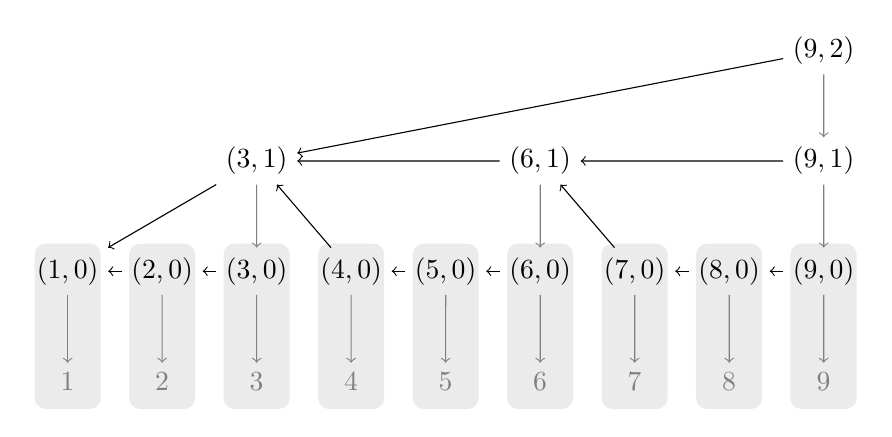
\begin{tikzpicture}[xscale=1.2,yscale=1.4]%[font=\tiny]
    % \useasboundingbox (-0.5,-1.5) rectangle (27.3,3.5);

	\pgfdeclarelayer{background}
	\pgfdeclarelayer{foreground}
	\pgfsetlayers{background,main,foreground}

	\begin{pgfonlayer}{foreground}
        \node[nodeItem] (n1) at (0, -1) {$1$};
        \node[nodeItem] (n2) at (1, -1) {$2$};
        \node[nodeItem] (n3) at (2, -1) {$3$};
        \node[nodeItem] (n4) at (3, -1) {$4$};
        \node[nodeItem] (n5) at (4, -1) {$5$};
        \node[nodeItem] (n6) at (5, -1) {$6$};
        \node[nodeItem] (n7) at (6, -1) {$7$};
        \node[nodeItem] (n8) at (7, -1) {$8$};
        \node[nodeItem] (n9) at (8, -1) {$9$};

        \node (v1_0) at (0, 0) {$(1, 0)$};
        \node (v2_0) at (1, 0) {$(2, 0)$};
        \node (v3_0) at (2, 0) {$(3, 0)$};
        \node (v3_1) at (2, 1) {$(3, 1)$};
        \node (v4_0) at (3, 0) {$(4, 0)$};
        \node (v5_0) at (4, 0) {$(5, 0)$};
        \node (v6_0) at (5, 0) {$(6, 0)$};
        \node (v6_1) at (5, 1) {$(6, 1)$};
        \node (v7_0) at (6, 0) {$(7, 0)$};
        \node (v8_0) at (7, 0) {$(8, 0)$};
        \node (v9_0) at (8, 0) {$(9, 0)$};
        \node (v9_1) at (8, 1) {$(9, 1)$};
        \node (v9_2) at (8, 2) {$(9, 2)$};

        \draw[myedge,edgeParent] (v1_0) -- (n1);
        \draw[myedge,edgeParent] (v2_0) -- (n2);
        \draw[myedge,edgeParent] (v3_0) -- (n3);
        \draw[myedge,edgeParent] (v4_0) -- (n4);
        \draw[myedge,edgeParent] (v5_0) -- (n5);
        \draw[myedge,edgeParent] (v6_0) -- (n6);
        \draw[myedge,edgeParent] (v7_0) -- (n7);
        \draw[myedge,edgeParent] (v8_0) -- (n8);
        \draw[myedge,edgeParent] (v9_0) -- (n9);

        \draw[edgePredecessor] (v3_1) -- (v3_0);
        \draw[edgePredecessor] (v6_1) -- (v6_0);
        \draw[edgePredecessor] (v9_1) -- (v9_0);
        \draw[edgePredecessor] (v9_2) -- (v9_1);

        \draw[skipEdge] (v2_0) -- (v1_0);
        \draw[skipEdge] (v3_0) -- (v2_0);
        \draw[skipEdge] (v3_1) -- (v1_0);
        \draw[skipEdge] (v4_0) -- (v3_1);
        \draw[skipEdge] (v5_0) -- (v4_0);
        \draw[skipEdge] (v6_0) -- (v5_0);
        \draw[skipEdge] (v6_1) -- (v3_1);
        \draw[skipEdge] (v7_0) -- (v6_1);
        \draw[skipEdge] (v8_0) -- (v7_0);
        \draw[skipEdge] (v9_0) -- (v8_0);
        \draw[skipEdge] (v9_1) -- (v6_1);
        \draw[skipEdge] (v9_2) -- (v3_1);
        
	\end{pgfonlayer}

    \begin{pgfonlayer}{main}
        % \begin{scope}[transparency group, opacity=0.2]
		% 	\draw[cPoolPath2,line width=11pt,rounded corners=0.1em,line cap=round] (v20_0.center) -- (v19_0.center) -- (v18_2.center) -- (v9_2.center) -- (v9_1.center) -- (v6_1.center) -- (v6_0.center);
		% 	\draw[cPoolPath2,line width=11pt,rounded corners=1em,line cap=round] (v20_0.center) -- (v19_0.center) -- (v18_2.center) -- (v9_2.center) -- (v9_1.center) -- (v6_1.center) -- (v6_0.center);
		% \end{scope}
	\end{pgfonlayer}

	\begin{pgfonlayer}{background}
		\newcommand{\onerecs}[1]{\draw[draw=none,rounded corners,fill=black,opacity=0.08] ($(#1,-1)-(0.35,0.25)$) rectangle ($({#1},0)+(0.35,0.25)$);}

		\foreach \x in {0,...,8}
		{
			\onerecs{\x};
		}

		% \newcommand{\tworecs}[1]{\draw[draw=none,rounded corners,fill=black,opacity=0.03] ($(#1,-1)-(0.4,0.3)$) rectangle ($({#1+2},1)+(0.4,0.3)$);}

		% \foreach \x in {0,...,15}
		% {
		% 	\tworecs{3*\x};
		% }

		% \newcommand{\fourrecs}[1]{\draw[draw=none,rounded corners,fill=black,opacity=0.03] ($(#1,-1)-(0.44,0.4)$) rectangle ($({#1+8},2)+(0.44,0.4)$);}

		% \foreach \x in {0,...,6}
		% {
		% 	\fourrecs{9*\x};
		% }

		% \newcommand{\eightrecs}[1]{\draw[draw=none,rounded corners,fill=black,opacity=0.02] ($(#1,-1)-(0.48,0.45)$) rectangle ($({#1+26},3)+(0.48,0.45)$);}

		% \foreach \x in {0,...,1}
		% {
		% 	\eightrecs{27*\x};
		% }
	\end{pgfonlayer}
\end{tikzpicture}

\end{document}